\documentclass[landscape,a1paper,fontscale=0.42]{baposter}

\usepackage[vlined]{algorithm2e}
\usepackage{times}
\usepackage{calc}
\usepackage{url}
\usepackage{graphicx}
\usepackage{amsmath}
\usepackage{amssymb}
\usepackage{relsize}
\usepackage{multirow}
\usepackage{booktabs}

\usepackage{graphicx}
\usepackage{multicol}
\usepackage[T1]{fontenc}
\usepackage{ae}
\usepackage{bm}

\usepackage{subcaption}
\usepackage{varwidth}
\usepackage{mathtools}
\usepackage{siunitx}
\usepackage{tabularx}
% \usepackage{tabularx}

\graphicspath{{images/}}

% Here, you can define your own macros. Some examples are given below.

% \newcommand{\R}[0]{\mathds{R}} % real numbers
% \newcommand{\Z}[0]{\mathds{Z}} % integers
% \newcommand{\N}[0]{\mathds{N}} % natural numbers
% \newcommand{\C}[0]{\mathds{C}} % complex numbers
% \renewcommand{\vec}[1]{{\boldsymbol{{#1}}}} % vector
% \newcommand{\mat}[1]{{\boldsymbol{{#1}}}} % matrix

% % -------- THEOREM ENVIRONMENTS --------

% \newtheoremstyle{break}
%   {\topsep}{\topsep}%
%   {\itshape}{}%
%   {\bfseries}{}%
%   {\newline}{}%
% % \theoremstyle{break}

% \theoremstyle{plain}
% \newtheorem{thm}{Theorem}[section] % reset theorem numbering for each chapter
% \newtheorem{prop}{Property}[section]
% \newtheorem{pstion}{Proposition}[section]
% \newtheorem{lemma}{Lemma}[section]

% \theoremstyle{definition}
% \newtheorem{defn}[thm]{Definition} % definition numbers are dependent on theorem numbers
% \newtheorem{exmp}[thm]{Example} % same for example numbers

% \theoremstyle{break}
% \newtheorem{lbdefn}[thm]{Definition} % Definition with line break after header

% ---------------------------------------

% Custom citation

\newcommand*\mycite[1]{\citet{#1} (\citeyear{#1})}

%%%%%%%%%%%%%%%%%%%%%%%%%%%%%%%%%%%%%%%%%
% Typography for vectors, matrices and tensors
%%%%%%%%%%%%%%%%%%%%%%%%%%%%%%%%%%%%%%%%%

\newcommand*\mat[1]{\mathbf{#1}}
\newcommand*\vv[1]{\mathbf{#1}}
\newcommand*\ten[1]{\bm{\mathcal{#1}}}

%%%%%%%%%%%%%%%%%%%%%%%%%%%%%%%%%%%%%%%%%
% Commands for operators
%%%%%%%%%%%%%%%%%%%%%%%%%%%%%%%%%%%%%%%%%

\newcommand{\grad}{\nabla}
\newcommand{\shrink}{\mathcal{S}}
\newcommand{\vvec}{\mathrm{vec}}
% \newcommand{\dim}{\mathrm{vec}}

\newcommand*\fold[1]{\mathrm{fold}(#1)}
\newcommand*\tr[1]{\mathrm{tr} \left[ #1 \right]}
\newcommand*\trr{\mathrm{tr}}

\newcommand*\mean[1]{\langle #1 \rangle}
\newcommand*\inner[2]{\langle #1, \, #2 \rangle}

\newcommand*\trp[1]{ #1^{\mathsf{T}} }

\newcommand*\inv[1]{ #1^{-1} }
\newcommand*\pinv[1]{ #1^{\dagger} }

\newcommand*\sprox[3]{\mathrm{prox}_{#1 #2}(#3)}
\newcommand*\prox[2]{\mathrm{prox}_{#1}(#2)}

\newcommand*\KL[2]{\mathrm{KL}(#1 || #2)}

\newcommand{\bvec}{\mathrm{bvec}}
\newcommand{\bvfold}{\mathrm{bvfold}}
\newcommand{\bdiag}{\mathrm{bdiag}}
\newcommand{\bdfold}{\mathrm{bdfold}}
\newcommand{\bcirc}{\mathrm{bcirc}}

\newcommand*\rk[1]{\mathrm{rank}(#1)}
\newcommand*\spn[1]{\mathrm{Span}(#1)}

% \newcommand*\argmin[1]{\mathrm{arg}\!\min_{#1}}
% \newcommand*\argmax[1]{\mathrm{arg}\!\max_{#1}}
\DeclareMathOperator*{\argmin}{argmin}
%%%%%%%%%%%%%%%%%%%%%%%%%%%%%%%%%%%%%%%%
% Notational shortcuts
%%%%%%%%%%%%%%%%%%%%%%%%%%%%%%%%%%%%%%%%%

\newcommand{\const}{\mathrm{const}}
\newcommand{\st}{\mathrm{s.t}}

\newcommand{\RR}{\mathbb{R}}
\newcommand{\Ga}{\mathrm{Ga}}
\newcommand{\var}{\mathrm{var}}

\newcommand{\bepsilon}{\bm{\epsilon}}
\newcommand{\bSigma}{\bm{\Sigma}}
\newcommand{\bLambda}{\bm{\Lambda}}
\newcommand{\bmu}{\bm{\mu}}

% \newcommand{\ie}{\textit{i.e,}~}
% \newcommand{\eg}{\textit{e.g,}~}

%%%%%%%%%%%%%%%%%%%%%%%%%%%%%%%%%%%%%%%%
% Norms
%%%%%%%%%%%%%%%%%%%%%%%%%%%%%%%%%%%%%%%%%

\newcommand*\Fro[1]{ || #1 ||_{\mathrm{F}} }
\newcommand*\Nuc[1]{ || #1 ||_{*} }
\newcommand*\One[1]{ || #1 ||_{1} }
\newcommand*\Two[1]{ || #1 ||_{2} }
\newcommand*\Twosq[1]{ || #1 ||_{2}^2 }
\newcommand*\LTwo[1]{ || #1 ||_{\mathrm{\ltwo}} }
\newcommand*\OneTwo[1]{ || #1 ||_{\lonetwo} }
\newcommand*\Frosq[1]{ || #1 ||_{\mathrm{F}}^2 }

\newcommand{\ltwo}{\ell_2}
\newcommand{\lone}{\ell_1}
\newcommand{\lzero}{\ell_0}
\newcommand{\linf}{\ell_{\infty}}
\newcommand{\lp}{\ell_p}
\newcommand{\lpq}{\ell_p / \ell_q}
\newcommand{\lonetwo}{\ell_1 / \ell_2}
\newcommand{\loneinf}{\ell_1 / \ell_{\infty}}

%%%%%%%%%%%%%%%%%%%%%%%%%%%%%%%%%%%%%%%%
% Matrices and elements for the Bayesian model
%%%%%%%%%%%%%%%%%%%%%%%%%%%%%%%%%%%%%%%%%

\newcommand{\A}{\mat{A}}
\newcommand{\At}{\trp{\A}}
\newcommand{\B}{\mat{B}}
\newcommand{\Bt}{\trp{\B}}
\newcommand{\C}{\mat{C}}
\newcommand{\D}{\mat{D}}
\newcommand{\R}{\mat{R}}

\newcommand{\X}{\mat{X}}
\newcommand{\Y}{\mat{Y}}
\newcommand{\Z}{\mat{Z}}
\newcommand{\T}{\mat{T}}
\newcommand{\E}{\mat{E}}
\newcommand{\LL}{\mat{\Lambda}}
\newcommand{\II}{\mat{I}}
\newcommand{\K}{\mat{K}}
\newcommand{\U}{\mat{U}}
\newcommand{\V}{\mat{V}}
\newcommand{\M}{\mat{M}}
\newcommand{\W}{\mat{W}}
\newcommand{\mS}{\mat{S}}


\newcommand{\aij}{\alpha^n_{i,j}}
\newcommand{\iaij}{\inv{{\aij}}}
\newcommand{\enij}{e^n_{i,j}}
\newcommand{\Ynij}{\Y^n_{i,j}}
\newcommand{\wni}{\vv{w}_{ni}}

\newcommand{\Tn}{\mat{T}_n}
\newcommand{\Tnt}{\trp{\Tn}}

\newcommand{\En}{\mat{E}_n}
\newcommand{\Ent}{\trp{\En}}
\newcommand{\Xn}{\mat{X}_n}
\newcommand{\Xnt}{\trp{\Xn}}
\newcommand{\Yn}{\mat{Y}_n}
\newcommand{\Ynt}{\trp{\Yn}}
\newcommand{\Wn}{\mat{W}_n}
\newcommand{\Wnt}{\trp{\Wn}}
\newcommand{\LLn}{\mat{\Lambda}_n}
\newcommand{\Kn}{\mat{K}_n}

\newcommand{\Ri}{\mat{R}_i}
\newcommand{\Rit}{\trp{\Ri}}

\newcommand{\Ei}{\mat{E}_i}
\newcommand{\Eit}{\trp{\Ei}}
\newcommand{\XXi}{\mat{X}_i}
\newcommand{\Xit}{\trp{\XXi}}
\newcommand{\Yi}{\mat{Y}_i}
\newcommand{\Yit}{\trp{\Yi}}
\newcommand{\Wi}{\mat{W}_i}
\newcommand{\Wit}{\trp{\Wi}}
\newcommand{\LLi}{\mat{\Lambda}_i}
\newcommand{\Ki}{\mat{K}_i}



\newcommand{\Uc}{\mat{U_c}}
\newcommand{\Uct}{\trp{\Uc}}
\newcommand{\Ur}{\mat{U_r}}
\newcommand{\Urt}{\trp{\Ur}}

\newcommand{\mbeta}{\mean{\beta}}
\newcommand{\maij}{\mean{\aij}}
\newcommand{\mgami}{\mean{\gamma_i}}

\newcommand{\mEn}{\mean{\En}}
\newcommand{\mUc}{\mean{\Uc}}
\newcommand{\mUr}{\mean{\Ur}}
\newcommand{\mTn}{\mean{\Tn}}

\newcommand{\mEnt}{\trp{\mEn}}
\newcommand{\mUct}{\trp{\mUc}}
\newcommand{\mUrt}{\trp{\mUr}}
\newcommand{\mTnt}{\trp{\mTn}}

\newcommand{\smbeta}{\sqrt{\mean{\beta}}}

\newcommand{\uci}{\vv{u}_{ci}}
\newcommand{\uri}{\vv{u}_{ri}}

%%%%%%%%%%%%%%%%%%%%%%%%%%%%%%%%%%%%%%%%%
%%          TENSOR NOTATIONS           %%
%%%%%%%%%%%%%%%%%%%%%%%%%%%%%%%%%%%%%%%%%
\newcommand{\tX}{\ten{X}}
\newcommand{\tS}{\ten{S}}
\newcommand{\tE}{\ten{E}}
\newcommand{\tL}{\ten{L}}
\newcommand{\tT}{\ten{T}}
\newcommand{\tG}{\ten{G}}
\newcommand{\tW}{\ten{W}}
\newcommand{\tO}{\ten{O}}
\newcommand{\tY}{\ten{Y}}
\newcommand{\tM}{\ten{M}}
\newcommand{\tI}{\ten{I}}
\newcommand{\tK}{\ten{K}}
\newcommand{\tR}{\ten{R}}

\newcommand*\matr[2]{\mathbf{#1}_{[#2]}}
\newcommand*\fslice[2]{\mathbf{#1}^{(#2)}}
\newcommand*\facmat[2]{\mathbf{#1}^{(#2)}}

%%%%%%%%%%%%%%%

\newcommand\Tstrut{\rule{0pt}{2.6ex}}         % = `top' strut
\newcommand\Bstrut{\rule[-0.9ex]{0pt}{0pt}}   % = `bottom' strut


% Paragraph
\newcommand*\mypar[1]{\vspace{0.5em} \noindent \textbf{#1} \hspace{0.5em}}

\makeatletter
\DeclareRobustCommand\onedot{\futurelet\@let@token\@onedot}
\def\@onedot{\ifx\@let@token.\else.\null\fi\xspace}

\def\eg{\emph{e.g}\onedot} \def\Eg{\emph{E.g}\onedot}
\def\ie{\emph{i.e}\onedot} \def\Ie{\emph{I.e}\onedot}
\def\cf{\emph{c.f}\onedot} \def\Cf{\emph{C.f}\onedot}
\def\etc{\emph{etc}\onedot} \def\vs{\emph{vs}\onedot}
\def\wrt{w.r.t\onedot} \def\dof{d.o.f\onedot}
\def\etal{\emph{et al}\onedot}
\makeatother

%%%%%%%%%%%%%%%%%%%%%%%%%%%%%%%%%%%%%%%%%%%%%%%%%%%%%%%%%%%%%%%%%%%%%%%%%%%%%
%% Begin of Document
%%%%%%%%%%%%%%%%%%%%%%%%%%%%%%%%%%%%%%%%%%%%%%%%%%%%%%%%%%%%%%%%%%%%%%%%%%%%%
\begin{document}\vspace*{-1mm}
%%%%%%%%%%%%%%%%%%%%%%%%%%%%%%%%%%%%%%%%%%%%%%%%%%%%%%%%%%%%%%%%%%%%%%%%%%%%%
%% Here starts the poster
%%---------------------------------------------------------------------------
%% Format it to your taste with the options
%%%%%%%%%%%%%%%%%%%%%%%%%%%%%%%%%%%%%%%%%%%%%%%%%%%%%%%%%%%%%%%%%%%%%%%%%%%%%
\begin{poster}{
 % Show grid to help with alignment
 grid=false,
 % Column spacing
 colspacing=0.7em,
 % Color style
 headerColorOne=cyan!20!white!90!black,
 borderColor=cyan!30!white!90!black,
 % Format of textbox
 textborder=faded,
 % Format of text header
 headerborder=open,
 headershape=roundedright,
 headershade=plain,
 background=none,
 bgColorOne=cyan!10!white,
 headerheight=0.12\textheight}
 % Eye Catcher
 {
      \includegraphics[width=0.205\linewidth]{iccv}
 }
 % Title
 {\sc\Huge Robust Kronecker Component Analysis}
%  {\sc\huge Robust Kronecker-Decomposable Component Analysis for Low-Rank Modeling}
 % Authors
 {Mehdi Bahri, Yannis Panagakis, and Stefanos Zafeiriou\\[1em]
 {\texttt{\{mehdi.bahri15, i.panagakis, s.zafeiriou\}@imperial.ac.uk}}}
 % University logo
 {
  \begin{tabular}{r}
    \includegraphics[width=0.22\textheight]{logo}
  \end{tabular}
 }

%%%%%%%%%%%%%%%%%%%%%%%%%%%%%%%%%%%%%%%%%%%%%%%%%%%%%%%%%%%%%%%%%%%%%%%%%%%%%%
%%% Now define the boxes that make up the poster
%%%---------------------------------------------------------------------------
%%% Each box has a name and can be placed absolutely or relatively.
%%% The only inconvenience is that you can only specify a relative position 
%%% towards an already declared box. So if you have a box attached to the 
%%% bottom, one to the top and a third one which should be inbetween, you 
%%% have to specify the top and bottom boxes before you specify the middle 
%%% box.
%%%%%%%%%%%%%%%%%%%%%%%%%%%%%%%%%%%%%%%%%%%%%%%%%%%%%%%%%%%%%%%%%%%%%%%%%%%%%%

%%%%%%%%%%%%%%%%%%%%%%%%%%%%%%%%%%%%%%%%%%%%%%%%%%%%%%%%%%%%%%%%%%%%%%%%%%%%%%
  \headerbox{Contribution: Robust Dictionaries and Tensor Factorization}{name=contribution,column=0,row=0,span=2}{
%%%%%%%%%%%%%%%%%%%%%%%%%%%%%%%%%%%%%%%%%%%%%%%%%%%%%%%%%%%%%%%%%%%%%%%%%%%%%%
%   We present a method for learning compact sparse representations in a noisy setting that combines ideas from dictionary learning and robust low-rank modeling. By imposing a separable dictionary we achieve scalability and exhibit links with tensor factorizations. Experimental assessment shows improvements of up to 16\% on image denoising benchmarks, and competitive background subtraction performance.
We present a method for learning compact sparse representations in a noisy setting that:
\begin{itemize}
    \item Combines dictionary learning and low-rank tensor factorizations
    \item Improves of up to 16\% over the state of the art on image denoising tasks
    \item Offers competitive background subtraction performance
\end{itemize}
  
% \vspace{1em}
  
%   Work first presented at ICCV 2017 \cite{Bahri2017} and extended in \cite{Bahri2018} (in review for IEEE TPAMI).
  }
%%%%%%%%%%%%%%%%%%%%%%%%%%%%%%%%%%%%%%%%%%%%%%%%%%%%%%%%%%%%%%%%%%%%%%%%%%%%%%
  \headerbox{Two equivalent views}{name=abstract,column=0,below=contribution}{
%%%%%%%%%%%%%%%%%%%%%%%%%%%%%%%%%%%%%%%%%%%%%%%%%%%%%%%%%%%%%%%%%%%%%%%%%%%%%%
    % Decompose $N$ observations $\vv{x}_i \in \RR^{mn}$ on $\D = \begin{bmatrix} \B \otimes \A & \II \end{bmatrix} \in \RR^{mn \times d}$ with representations $\vv{y}_i = \trp{\begin{bmatrix}\vv{r}_i & \vv{e}_i\end{bmatrix}}  \in \RR^{d}$:% through a two-level structured regularized sparse dictionary learning problem:
    % \begin{align}
    %   \label{eq:dict_learning}
    %   \min_{\D, \mat{Y}}{ \sum_i \Twosq{\vv{x}_i - \D \vv{y}_i } } + \lambda \sum_i \One{\vv{y}_i} + \Fro{\D}
    % \end{align}

    % \begin{itemize}
    %   \item $\vv{e}_i \in \RR^{mn}$: outliers (gross corruption)
    %   \item $\vv{r}_i \in \RR^{r^2}$: codes learnt w.r.t. a Kronecker dictionary $\B \otimes \A$ with $\A \in \RR^{m \times r}, \B \in \RR^{n \times r}$
    % \end{itemize}    

    We show learning some structured dictionaries is equivalent to factorizing \textbf{3D tensors}:
    \begin{align}\label{eq:constrained_pb}
       \begin{matrix*}[l]
       \min_{\ten{L}, \ten{E}} & f(\ten{L}) + \lambda \One{\tE}\\
       \st & \tX = \ten{L} + \tE
       %\st & \forall i, \; \XXi = \A \Ri \Bt + \Ei
       \end{matrix*}
   \end{align}
   
   We consider \textbf{Kronecker dictionaries} $\D = \B \otimes \A$.
   
   \vspace{1em}
   
   Why? Work with images in matrix form:
   \begin{itemize}
    \item Preserves the spatial structure of images
    \item Allows to solve matrix equations efficiently
    \item Stacking the matrices as a 3D array gives a \textbf{3-way tensor}
   \end{itemize}
    
}



 %%%%%%%%%%%%%%%%%%%%%%%%%%%%%%%%%%%%%%%%%%%%%%%%%%%%%%%%%%%%%%%%%%%%%%%%%%%%%%
\headerbox{Background subtraction experiments}{name=speed,column=2,row=0,span=2}{
 %%%%%%%%%%%%%%%%%%%%%%%%%%%%%%%%%%%%%%%%%%%%%%%%%%%%%%%%%%%%%%%%%%%%%%%%%%%%%%
 
  \begin{tabular}{c@{\hspace{0.05em}}c@{\hspace{0.1em}}c@{\hspace{0.1em}}c@{\hspace{0.1em}}c@{\hspace{1em}}c@{\hspace{0.1em}}c@{\hspace{0.1em}}c@{\hspace{0.1em}}c@{\hspace{0.1em}}c}
    \multicolumn{5}{c}{\smaller \textit{Airport Hall - Frame 1}}\\[-0.2em]
    \includegraphics[width=0.093\linewidth]{Ref/hall_1_original}            &
    \includegraphics[width=0.093\linewidth]{Ref/hall_fg_1_original}         &
    \includegraphics[width=0.093\linewidth]{BG_hall/hall_bg_1_cauchy_st}    &
    \includegraphics[width=0.093\linewidth]{BG_hall/hall_bg_1_welsh_st}     &
    \includegraphics[width=0.093\linewidth]{BG_hall/hall_bg_1_tnn}      \\
    \smaller[5] Original & \smaller[5] GT & \smaller[5] Cauchy ST & \smaller[5] Welsh ST & \smaller[5] TRPCA '16\\
    %
     
    \includegraphics[width=0.093\linewidth]{BG_hall/hall_bg_1_horpca_s}     &
    \includegraphics[width=0.093\linewidth]{BG_hall/hall_bg_1_nctrpca}      &
    \includegraphics[width=0.093\linewidth]{BG_hall/hall_bg_1_rnndl}        &
    \includegraphics[width=0.093\linewidth]{BG_hall/hall_bg_1_rpca}         &
    \includegraphics[width=0.093\linewidth]{BG_hall/hall_bg_1_rpca2d_l1}
    \\[-0.1em]
    \smaller[5] HORPCA-S & \smaller[5] NCTRPCA & \smaller[5] RNNDL & \smaller[5] RPCA & \smaller[5] RKCA (1)\\
  \end{tabular}
  \begin{tabular}{c@{\hspace{0.05em}}c@{\hspace{0.1em}}c@{\hspace{0.1em}}c@{\hspace{0.1em}}c@{\hspace{1em}}c@{\hspace{0.1em}}c@{\hspace{0.1em}}c@{\hspace{0.1em}}c@{\hspace{0.1em}}c}
    \multicolumn{5}{c}{\smaller \textit{Highway - Frame 105}}\\[-0.2em]
    \includegraphics[width=0.093\linewidth]{Ref/highway_bg_105_original}            &
    \includegraphics[width=0.093\linewidth]{Ref/highway_fg_105_original}            &
    \includegraphics[width=0.093\linewidth]{BG_highway/highway_bg_105_cauchy_st}    &
    \includegraphics[width=0.093\linewidth]{BG_highway/highway_bg_105_welsh_st}     &
    \includegraphics[width=0.093\linewidth]{BG_highway/highway_bg_105_tnn} &
    
    \\
     \smaller[5] Original & \smaller[5] GT & \smaller[5] Cauchy ST & \smaller[5] Welsh ST & \smaller[5] TRPCA '16\\
    %
    \includegraphics[width=0.093\linewidth]{BG_highway/highway_bg_105_horpca_s}     &
    \includegraphics[width=0.093\linewidth]{BG_highway/highway_bg_105_nctrpca}      &
    \includegraphics[width=0.093\linewidth]{BG_highway/highway_bg_105_rnndl}        &
    \includegraphics[width=0.093\linewidth]{BG_highway/highway_bg_105_rpca}         &
    \includegraphics[width=0.093\linewidth]{BG_highway/highway_bg_105_rpca2d_l1}    &
    \\[-0.1em]
    \smaller[5] HORPCA-S & \smaller[5] NCTRPCA & \smaller[5] RNNDL & \smaller[5] RPCA & \smaller[5] RKCA (1) &\\
  \end{tabular}
 
 
  \begin{multicols}{2}
  \textbf{Procedure and results. }
  Panel of recent algorithms for robust component analysis compared on excerpts of the \textit{Highway} dataset, and of the \textit{Airport Hall} dataset (see \cite{Bahri2017}). We report the AUC scores. 
  
  \vspace{1em}
  Our model matched the best performance on the \textit{Highway} dataset and provided the highest performance on the \textit{Hall} benchmark.
  %An additional step for robust estimation of the mean image was used.

  \hspace{2em}
  \resizebox{0.8\columnwidth}{!}{
    \begin{tabular}{|c|c|c|}\hline
      \textbf{Algorithm} & \textbf{Highway} & \textbf{Hall} \\ \hline
      \textbf{RKCA (proposed)} & 0.94 & 0.88 \\ \hline
        TRPCA '16 & 0.94 & 0.86 \\ \hline
        NC TRPCA   & 0.93 & 0.86 \\ \hline
        \textit{RPCA (baseline)} & 0.94 & 0.85 \\ \hline
        \textit{RNNDL (baseline)} & 0.94 & 0.85\\ \hline
        \textit{LRR Exact (baseline)} & 0.94 & 0.84\\ \hline
        \textit{LRR Inexact (baseline)} & 0.93 & 0.84\\ \hline
        HORPCA-S  & 0.93 & 0.86 \\ \hline
        Cauchy ST & 0.83 & 0.76 \\ \hline
        Welsh ST & 0.82 & 0.71 \\ \hline
        TRPCA '14 & 0.76 & 0.61 \\ \hline
    \end{tabular}
  }
  \end{multicols}
   }
%
% %%%%%%%%%%%%%%%%%%%%%%%%%%%%%%%%%%%%%%%%%%%%%%%%%%%%%%%%%%%%%%%%%%%%%%%%%%%%%%
%   \headerbox{Methods Compared}{name=methods,column=0,below=algorithm}{
% %%%%%%%%%%%%%%%%%%%%%%%%%%%%%%%%%%%%%%%%%%%%%%%%%%%%%%%%%%%%%%%%%%%%%%%%%%%%%%
%   \begin{tabular}{rllllll}
%     Method                              & Hessian               &                                        & Gradient        &                                  & Speed      & Capture Range\\
%     \midrule
% \CoDe{} (this paper)                & Not used              &                                        & True:           & $\tilde{J}_{\qq_0}^T\e{\qq_0}$   & Fast       & Large  \\[0.1em]
% \LinCoDe{} (this paper)             & Not used              &                                        & Linear Approx:  & $\bar{J}^T\e{\qq_0}$             & Very Fast  & Medium \\[0.1em]
% \CoLiNe{}~\cite{burkhardt86:motion} & Constant Approx.:     & $\bar{J}^T\bar{J}$                     & True:           & $\tilde{J}_{\qq_0}^T\e{\qq_0}$   & Fast       & Medium \\[0.1em]
% \ICIA{}~\cite{matthews:aamr}        & Constant Approx.:     & $\bar{J}^T\bar{J}$                     & Linear Approx:  & $\bar{J}^T\e{\qq_0}$             & Very Fast  & Small  \\[0.1em]
% \CoNe{}~\cite{matthews:kanade20}    & Gauss-Newton Approx.: & $\tilde{J}_{\qq_0}^T\tilde{J}_{\qq_0}$ & True:           & $\tilde{J}_{\qq_0}^T\e{\qq_0}$   & Slow       & Large  
%   \end{tabular}
%   The methods introduced in this paper are Hessian-free gradient descent methods.
%  }
%

 %%%%%%%%%%%%%%%%%%%%%%%%%%%%%%%%%%%%%%%%%%%%%%%%%%%%%%%%%%%%%%%%%%%%%%%%%%%%%%
   \headerbox{Model structure}{name=data,column=0,above=bottom,below=abstract}{
 %%%%%%%%%%%%%%%%%%%%%%%%%%%%%%%%%%%%%%%%%%%%%%%%%%%%%%%%%%%%%%%%%%%%%%%%%%%%%%       

   
   {
  \hfill    \includegraphics[width=0.97\linewidth]{decomp} \hfill
   }
   
   \begin{itemize}
       \item Decompose $\XXi$ in  $\mat{L}_i = \A \Ri \Bt$ and outliers $\Ei$
       \item Dimension $r$ of \textbf{code} $\Ri$ bounds rank of each low-rank component
       \item Parameter sharing in $\A$ and $\B$ ensures the whole dataset is low-rank
   \end{itemize}
   
  \vspace{0.25em}
  Regularizers:
  \begin{itemize}
      \item (1) $f(\tL) = \lambda \One{\tR} + \Fro{\B \otimes \A}$
      \item (2) $f(\tL) = \lambda \One{\tR} \Fro{\B \otimes \A}$
  \end{itemize}
  
  Extension possible to tensor completion \cite{Bahri2018}.
  
%   Here we assume every observation is low rank + whole data set is low-rank at once + L such that Kronecker structure + use sparsity to encourage low-rankness.
   
%   Choice of f either give us fast algorithms with relaxation or theoretical guarantees.
  
%   In vision, observations are often vectorized matrices $\vv{x}_i = \vvec({\XXi}), \XXi \in \RR^{m \times n}$.
%   \vspace{1em}   
%   Matrix form:
%   \begin{itemize}
%     \item Preserves the spatial structure of images
%     \item Allows to solve matrix equations efficiently
%     \item Stacking the matrices as a 3D array gives a \textbf{3-way tensor}
%   \end{itemize}
   
%   \vspace{1em}
%   We show \cite{Bahri2017} (\ref{eq:dict_learning}) is equivalent to the tensor factorization:
%   \begin{equation}\label{eq:matrix_2d_rpca}
%   \begin{split}
%   \min_{\A, \B, \ten{R}, \ten{E}} \sum_i \Frosq{\XXi - \A \Ri \Bt - \Ei }  \\ 
%       + \lambda \sum_i \One{\Ri} + \lambda \sum_i \One{\Ei} + \Fro{\B \otimes \A}
%   \end{split}
%   \end{equation}
%   Or equivalently, as a structured tensor factorization:
%   \begin{align}\label{eq:constrained_pb}
%       \begin{matrix*}[l]
%       \min_{\A, \B, \ten{R}, \ten{E}} & \lambda \One{\ten{R}} + \lambda \One{\tE} + \Fro{\B \otimes \A}\\
%       \st & \tX = \ten{R} \times_1 \A \times_2 \B + \tE
%       %\st & \forall i, \; \XXi = \A \Ri \Bt + \Ei
%       \end{matrix*}
%   \end{align}
   %We set $r \leq \min(m, n)$ as a natural upper bound on the rank of the frontal slices of $\tL = \ten{R} \times_1 \A \times_2 \B$, and on its mode-$1$ and mode-$2$ ranks.
   
       
%     Observations often are unfolded matrices $\vv{x}_i = \vvec({\XXi}), \XXi \in \RR^{m \times n}$.
   
%   \vspace{1em}   
%   Matrix form:
%   \begin{itemize}
%     \item Preserves the spatial structure of images
%     \item Allows to solve matrix equations efficiently
%     \item Stacking the matrices as a 3D array gives a \textbf{3-way tensor}
%   \end{itemize}
   
%   {
%   \hfill    \includegraphics[width=0.97\linewidth]{decomp} \hfill
%   }
   
%   We show \cite{Bahri2017} (\ref{eq:dict_learning}) is equivalent to the tensor factorization:
%   \begin{align}\label{eq:constrained_pb}
%       \begin{matrix*}[l]
%       \min_{\A, \B, \ten{R}, \ten{E}} & \lambda \One{\ten{R}} + \lambda \One{\tE} + \Fro{\B \otimes \A}\\
%       \st & \tX = \ten{R} \times_1 \A \times_2 \B + \tE
%       %\st & \forall i, \; \XXi = \A \Ri \Bt + \Ei
%       \end{matrix*}
%   \end{align}
   
   }

 %%%%%%%%%%%%%%%%%%%%%%%%%%%%%%%%%%%%%%%%%%%%%%%%%%%%%%%%%%%%%%%%%%%%%%%%%%%%%%

\headerbox{Image denoising experiments on the Yale-B dataset}{name=tracking,column=2,span=2,below=speed,above=bottom}
{
  %%%%%%%%%%%%%%%%%%%%%%%%%%%%%%%%%%%%%%%%%%%%%%%%%%%%%%%%%%%%%%%%%%%%%%%%%%%%%%
  {
    \begin{tabular}{c@{\hspace{0.05em}}c@{\hspace{0.1em}}c@{\hspace{0.1em}}c@{\hspace{0.1em}}c@{\hspace{1em}}c@{\hspace{0.1em}}c@{\hspace{0.1em}}c@{\hspace{0.1em}}c@{\hspace{0.1em}}c@{\hspace{0.1em}}r}
    
      \multicolumn{5}{c}{\smaller \textit{30\% Salt \& Pepper noise}} & \multirow{5}{*}{\hspace{-0.2em}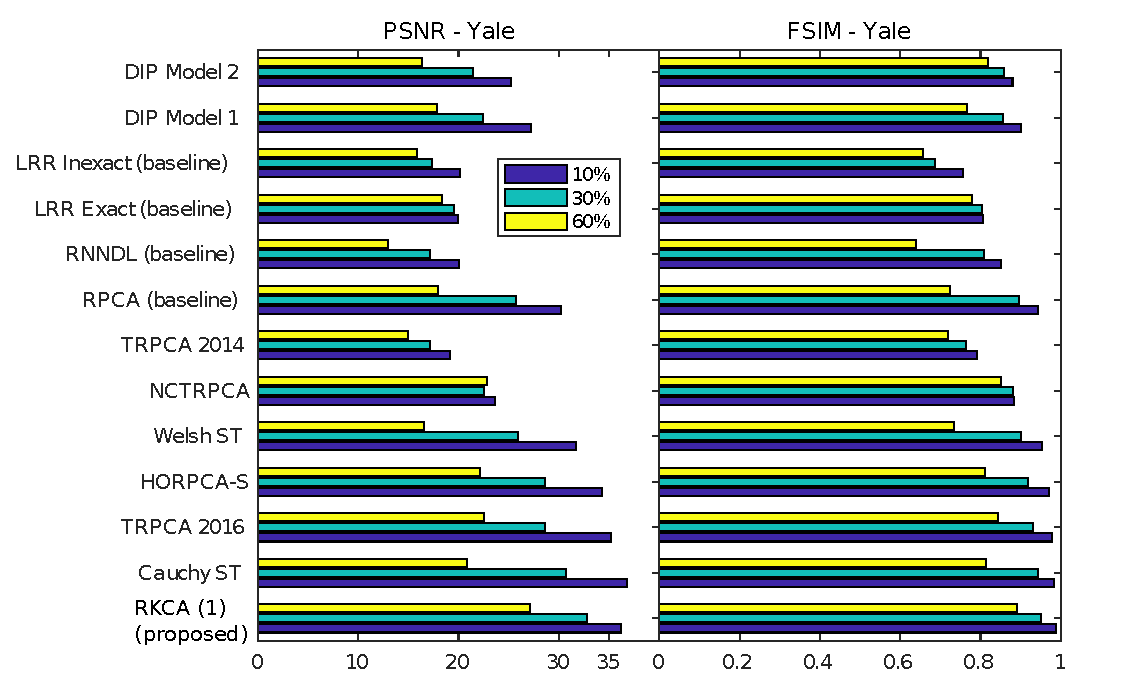
\includegraphics[width=.43\columnwidth]{side_by_side_psnr_fsim_yale_col}}\\[-0.2em]
      \includegraphics[height=0.12\linewidth]{Ref/yale_1_original}                 &
      \includegraphics[height=0.12\linewidth]{Ref/yale_1_03_original}              &
      \includegraphics[height=0.12\linewidth]{DN_yale/yale_03_1_cauchy_st_fsim}    &
      \includegraphics[height=0.12\linewidth]{DN_yale/yale_03_1_welsh_st_fsim}     &
      \includegraphics[height=0.12\linewidth]{DN_yale/yale_03_1_cvpr2016_tnn_fsim} &
      &\\
      \smaller[5] Original & \smaller[5] Noisy & \smaller[5] Cauchy ST & \smaller[5] Welsh ST & \smaller[5] TRPCA '16 & \\
      %
      \includegraphics[height=0.12\linewidth]{DN_yale/yale_03_1_horpca_s_fsim}     &
      \includegraphics[height=0.12\linewidth]{DN_yale/yale_03_1_nctrpca_fsim}      &
      \includegraphics[height=0.12\linewidth]{DN_yale/yale_03_1_rnndl_fsim}        &
      \includegraphics[height=0.12\linewidth]{DN_yale/yale_03_1_rpca_fsim}         &
      \includegraphics[height=0.12\linewidth]{DN_yale/yale_03_1_rpca2d_l1_fsim}
      &\\[-0.1em]
      \smaller[5] HORPCA-S & \smaller[5] NCTRPCA & \smaller[5] RNNDL & \smaller[5] RPCA & \smaller[5] RKCA (1)&
      
    \end{tabular}\hspace{-1em}
    
  }
  \vspace{-0.7em}
  \begin{multicols}{2}

    \textbf{Procedure and results.}
    % Keeping the 64 illuminations of the first subject \cite{Georghiades2001}, we expect the data tensor to be low-rank on all 3 modes. At 30\% noise and above, our method showed markedly higher quantitative scores and noticeably better reconstructions.
    On the 64 illuminations of first subject \cite{Bahri2017}, data tensor low-rank on all 3 modes.

    \vspace{1em}
    At noise $\geq 30\%$, we achieved markedly higher quantitative scores and noticeably better reconstructions.
    
    % We invite the reader to look at the texture of the skin, the white of the eye, and at the reflection of the light on the subject's skin and pupil. The latter, in particular, is very close in nature to the white pixel corruption of the salt \& pepper noise.
    Differences best seen on:
    \begin{itemize}
      \item Skin texture, white of eye
      \item Reflected light (pupil, skin)
    \end{itemize}
  \end{multicols}
}

%%%%%%%%%%%%%%%%%%%%%%%%%%%%%%%%%%%%%%%%%%%%%%%%%%%%%%%%%%%%%%%%%%%%%%%%%%%%%%
   \headerbox{Novelty of our approach}{name=lowrestracking,column=1,span=1,below=contribution,above=ncadmm}{
 %%%%%%%%%%%%%%%%%%%%%%%%%%%%%%%%%%%%%%%%%%%%%%%%%%%%%%%%%%%%%%%%%%%%%%%%%%%%%%
  Our model differs from classical tensor factorizations:
   \begin{itemize}
       \item Assume low-rankness of each slice and of the whole tensor simultaneously
       \item Use sparsity in $\tR$ to encourage low-rankness
       \item Regularize directly the factors and not the unfoldings
   \end{itemize}
 
%   Our algorithm successfuly recovers the components of (\ref{eq:constrained_pb}) on synthetic data.

%   \vspace{1em}

%   \hfill \begin{tabular}{c}
%     \includegraphics[width=.95\linewidth]{Synthetic/kdrsdl_sample_rank}\\
%     \textit{True ranks (42, 12) recovered, $r = 100$}\\
%     \vspace{0.5em}\\
%     \includegraphics[width=.95\linewidth]{Synthetic/synth_60_error_kdrsdl_2}\\
%     \textit{$\ell_2$ error on $\tL$, density of $\tE$, 60\% corruption}
%   \end{tabular} \hfill

  }

 %%%%%%%%%%%%%%%%%%%%%%%%%%%%%%%%%%%%%%%%%%%%%%%%%%%%%%%%%%%%%%%%%%%%%%%%%%%%%%%
  \headerbox{Solving the problem}{name=ncadmm,column=1,above=bottom}{
    % Problem (\ref{eq:constrained_pb}) is convex in each component but not jointly convex.
    Solve by (non) convex ADMM.
    \begin{itemize}
        \item Fast relaxation for regularizer (1) \cite{Bahri2017}
        \item Theoretical guarantees for regularizer (2) \cite{Bahri2018}
    \end{itemize}
    
    Experimental validation:
    
    \hfill \begin{tabular}{c}
    \includegraphics[width=.95\linewidth]{Synthetic/kdrsdl_sample_rank}\\
    \textit{True ranks (42, 12) recovered, $r = 100$}\\
    \vspace{0.5em}\\
    \includegraphics[width=.95\linewidth]{Synthetic/synth_60_error_kdrsdl_2}\\
    \textit{$\ell_2$ error on $\tL$, density of $\tE$, 60\% corruption}
  \end{tabular} \hfill
    
    Fast scalable implementation with LADMM.


%     % \vspace{1em}
%     % We optimize an upper bound on (\ref{eq:constrained_pb}) with $\Fro{\B \otimes \A} = \Fro{\A} \Fro{\B} \leq \frac{\Frosq{\A} + \Frosq{\B}}{2}$ for scalability and tractability. We introduce split variables $\Ki$ such that $\forall i, \; \Ki = \Ri$ and solve:

%     % \begin{align}\label{eq:constrained_pb_rpca_upper_bound}
%     %     \begin{matrix*}[l]
%     %     \displaystyle \min_{\A, \B, \ten{R}, \tK \ten{E}} & \lambda \One{\ten{R}} + \lambda \One{\tE} + \frac{1}{2}(\Frosq{\A} + \Frosq{\B})\\
%     %     \st & \tX = \ten{K} \times_1 \A \times_2 \B + \tE \\
%     %     \st & \tR = \tK
%     %     \end{matrix*}
%     % \end{align}
%  {
%   \hfill    \includegraphics[width=0.97\linewidth]{decomp} \hfill
%  }
%  \begin{itemize}
%   \item $\XXi, \Ri$, and $\Ei$ concatenated as the frontal slices of 3-way tensors
%   \item $r \leq \min(m, n)$ bounds the mode-$1$ and mode-$2$ ranks of $\tL = \ten{R} \times_1 \A \times_2 \B$
%  \end{itemize}
%  Min. bound via non-convex ADMM with splitting and $\Fro{\B \otimes \A} = \Fro{\A} \Fro{\B} \leq \frac{1}{2}\left( \Frosq{\A} + \Frosq{\B} \right)$.

  %Spliting allows for closed-form proximal operators and no fixed-point updates. The dual steps are bounded for convergence. 

 %%%%%%%%%%%%%%%%%%%%%%%%%%%%%%%%%%%%%%%%%%%%%%%%%%%%%%%%%%%%%%%%%%%%%%%%%%%%%%%
  % \begin{algorithm}[H]
  %   \dontprintsemicolon
  %   \linesnumbered
  %   \For{Blur and regularisation values}{
  %     \nl Initialize $\qq, \qq_{\text{best}}$ and $\kappa$\;
  %     \Repeat{converged}{
  %       \nl Calculate $\Nabla{\pp}{\tilde{F}(\qq,\VEC 0)}$, $F(\qq)$\;
  %       \eIf{$F(\qq) < F(\qq_{\text{best}})$}{
  %         %\nl Calculate distance between best warp estimate and current warp estimate to test for convergence\;
  %         \nl $\qq_{\text{best}} \gets \qq$\;
  %         %\If{More than three successiv updates}{ (Too much detail)
  %           \nl Increase $\kappa$\;
  %         %}
  %       }{
  %         \If{$\kappa$ smaller than threshold}{
  %           \nl return\;
  %         }%{
  %            decrease $\kappa$\;
  %         %}
  %       }
  %       \nl Calculate $\pp$ from $\Nabla{\pp}{\tilde{F}(\qq_{best},\pp)}$ and $\kappa$\;
  %       \nl $\qq \gets \C{\circ}{\qq, \pp}$
  %     }
  %   }
  % \end{algorithm}
   }

%%%%%%%%%%%%%%%%%%%%%%%%%%%%%%%%%%%%%%%%%%%%%%%%%%%%%%%%%%%%%%%%%%%%%%%%%%%%%%
\headerbox{References}{name=references,column=2, span=2, above=bottom}{
%%%%%%%%%%%%%%%%%%%%%%%%%%%%%%%%%%%%%%%%%%%%%%%%%%%%%%%%%%%%%%%%%%%%%%%%%%%%%%
  \smaller
  
  \bibliographystyle{ieee}
  \renewcommand{\section}[2]{\vskip 0.05em}
    \begin{thebibliography}{1}\itemsep=-0.01em
    \setlength{\baselineskip}{0.4em}

    % \bibitem{Goyette2012}
    % N. Goyette, P. M. Jodoin, F. Porikli, J. Konrad, and P. Ish-war.
    % \newblock changedetection.net:  A new change detection benchmark dataset.
    % \newblock In IEEE  Computer  Society  Conference  on Computer Vision and Pattern Recognition Workshops, 2012.

    % \bibitem{Li2004}
    % L. Li, W. Huang, I.-H. Gu, and Q. Tian.
    % \newblock Statistical Modeling of Complex Backgrounds for Foreground Object Detection.
    % \newblock In IEEE Transactions on Image Processing, 11 2004.

    % \bibitem{Georghiades2001}
    % A. Georghiades, P. Belhumeur, and D. Kriegman.
    % \newblock From few to many:  illumination cone models for face recognition under variable lighting and pose. 
    % \newblock In IEEE Transactions on Pattern Analysis and Machine Intelligence, 6 2001.
    
    \bibitem{Bahri2017}
    M. Bahri, Y. Panagakis, and S. Zafeiriou.
    \newblock Robust Kronecker-Decomposable Component Analysis for Low-Rank Modeling.
    \newblock The IEEE International Conference on Computer Vision (ICCV), 10 2017.

    \bibitem{Bahri2018}
    M. Bahri, Y. Panagakis, and S. Zafeiriou.
    \newblock Robust Kronecker Component Analysis.
    \newblock arXiv preprint 1801.06432 (in review for IEEE TPAMI), 1 2018.

    \end{thebibliography}
}


\end{poster}%
%
\end{document}
